\section*{Current Progress}

Overview of the progress made since the first milestone is as follows:

\begin{itemize}[leftmargin=1.5em]
	\item \textbf{Pipeline refactoring into a callable API:}
	The verification flow is now exposed through \texttt{CHC\_Verification(\ldots)}
	with structured output fields (status, advice, timing, and per-property results)
	instead of an interactive-only CLI path.

	\item \textbf{Optimization pipeline added:}
	A \texttt{BASIC} optimization mode adds static IR analysis, turn-safety reasoning,
	and summarizable-loop compression before CHC querying, while
	\texttt{OptimizationLevel.NONE} retains the conservative baseline behavior.

	\item \textbf{Property scope feature added:}
	Properties can now be checked over all reachable states or restricted to
	terminating states only (\texttt{property\_scope = "terminating"}).

	\item \textbf{Heading-grid safety checks integrated:}
	The verifier now models and queries heading-grid safety explicitly through
	a dedicated \texttt{BadHeading} relation before property checking.

	\item \textbf{Heading-grid hints integrated:}
	Users can either request verification of the heading-grid invariant
	(\texttt{check\_heading\_always\_on\_grid}) or force an assumption
	(\texttt{heading\_on\_grid\_always}) for faster runs on hard cases.

	\item \textbf{Correctness tests:}
	\textit{TODO}
	

	\item \textbf{Performance tests:}
	\textit{TODO}
\end{itemize}

See \autoref{fig:main_pipeline_flow} for a visual overview of the main verification pipeline stages, responsibilities, and data flow, and the subsequent sections for detailed implementation notes on each major feature addition and refactor.
The details of correctness and performance testing can be found in the \hyperref[sec:tests]{Tests section}.

\subsection*{Main Pipeline Flow (Responsibilities and Data Flow)}

\begin{figure}[h]
\centering
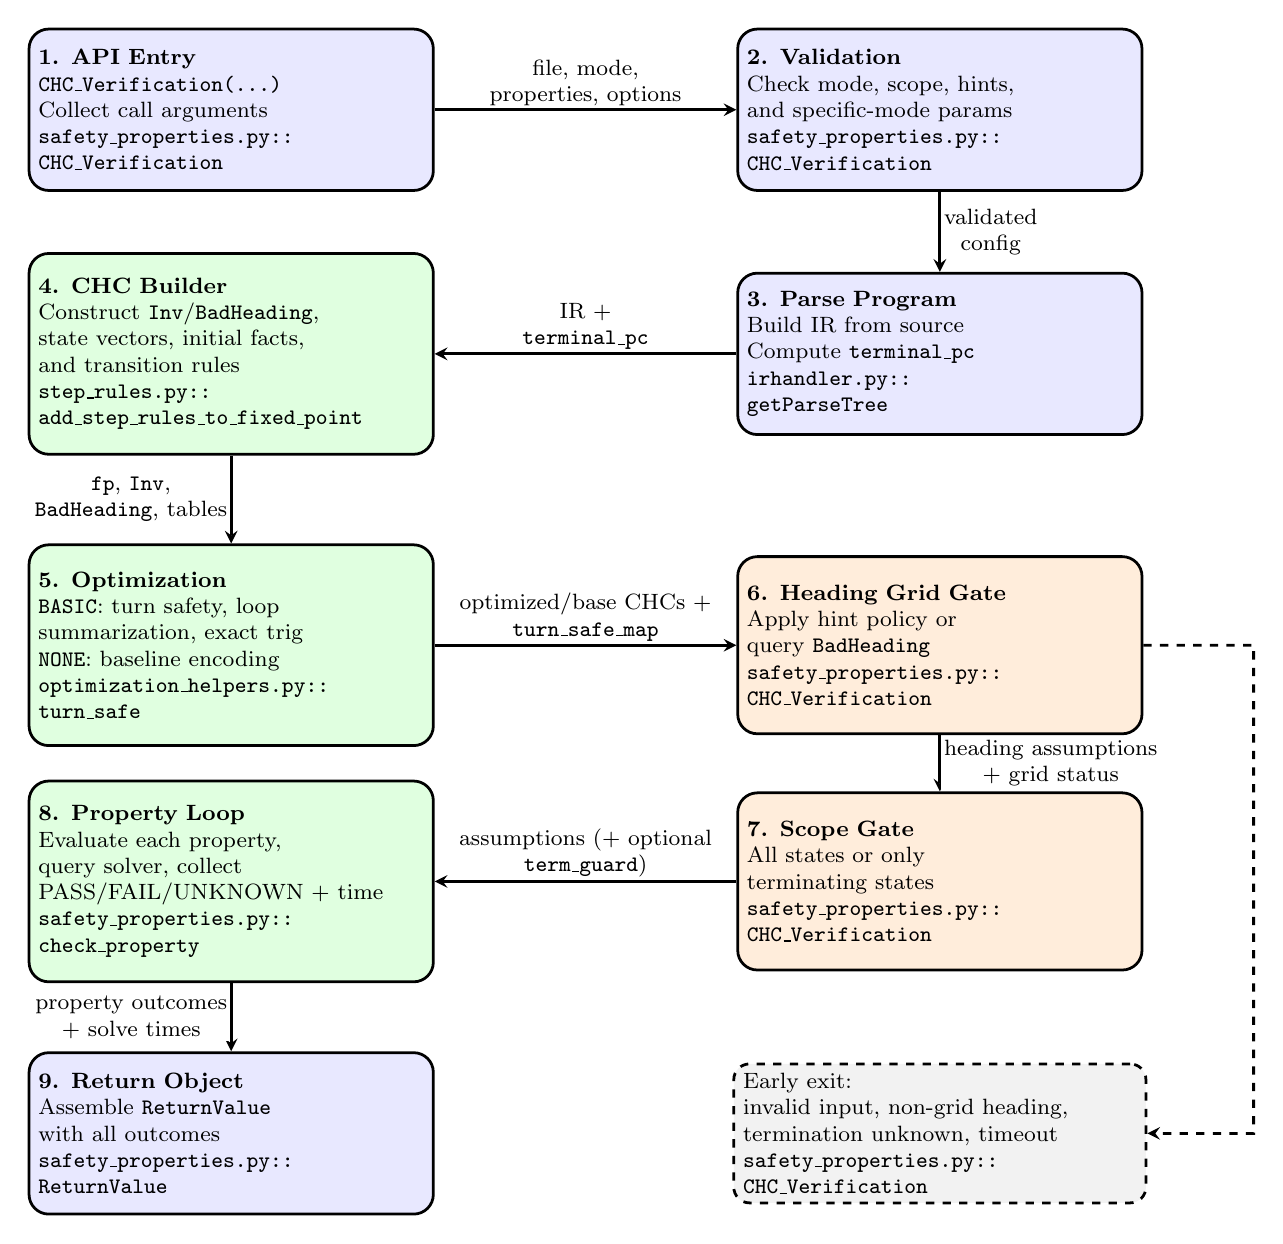
\begin{tikzpicture}[>=stealth, line width=1pt, font=\footnotesize]
\tikzset{
	stage/.style={draw, rounded corners=2.5mm, align=left, text width=4.9cm, minimum height=2.05cm, fill=blue!9},
	heavy/.style={draw, rounded corners=2.5mm, align=left, text width=4.9cm, minimum height=2.55cm, fill=green!12},
	gate/.style={draw, rounded corners=2.5mm, align=left, text width=4.9cm, minimum height=2.25cm, fill=orange!14}
}

% Two-column layout (snake flow)
\node[stage] (n1) at (0,0)
{\textbf{1. API Entry}\\
\texttt{CHC\_Verification(\ldots)}\\
Collect call arguments\\
\texttt{safety\_properties.py::\\CHC\_Verification}};

\node[stage] (n2) at (9.0,0)
{\textbf{2. Validation}\\
Check mode, scope, hints,\\
and specific-mode params\\
\texttt{safety\_properties.py::\\CHC\_Verification}};

\node[stage] (n3) at (9.0,-3.1)
{\textbf{3. Parse Program}\\
Build IR from source\\
Compute \texttt{terminal\_pc}\\
\texttt{irhandler.py::\\getParseTree}};

\node[heavy] (n4) at (0,-3.1)
{\textbf{4. CHC Builder}\\
Construct \texttt{Inv}/\texttt{BadHeading},\\
state vectors, initial facts,\\
and transition rules\\
\texttt{step\_rules.py::\\add\_step\_rules\_to\_fixed\_point}};

\node[heavy] (n5) at (0,-6.8)
{\textbf{5. Optimization}\\
\texttt{BASIC}: turn safety, loop\\
summarization, exact trig\\
\texttt{NONE}: baseline encoding\\
\texttt{optimization\_helpers.py::\\turn\_safe}};

\node[gate] (n6) at (9.0,-6.8)
{\textbf{6. Heading Grid Gate}\\
Apply hint policy or\\
query \texttt{BadHeading}\\
\texttt{safety\_properties.py::\\CHC\_Verification}};

\node[gate] (n7) at (9.0,-9.8)
{\textbf{7. Scope Gate}\\
All states or only\\
terminating states\\
\texttt{safety\_properties.py::\\CHC\_Verification}};

\node[heavy] (n8) at (0,-9.8)
{\textbf{8. Property Loop}\\
Evaluate each property,\\
query solver, collect\\
PASS/FAIL/UNKNOWN + time\\
\texttt{safety\_properties.py::\\check\_property}};

\node[stage] (n9) at (0,-13.0)
{\textbf{9. Return Object}\\
Assemble \texttt{ReturnValue}\\
with all outcomes\\
\texttt{safety\_properties.py::\\ReturnValue}};

% Arrows with data flow labels
\draw[->] (n1.east) -- node[above, align=center, fill=white, inner sep=1pt] {file, mode,\\properties, options} (n2.west);
\draw[->] (n2.south) -- node[right, align=center, fill=white, inner sep=1pt] {validated\\config} (n3.north);
\draw[->] (n3.west) -- node[above, align=center, fill=white, inner sep=1pt] {IR +\\\texttt{terminal\_pc}} (n4.east);
\draw[->] (n4.south) -- node[left, align=center, fill=white, inner sep=1pt] {\texttt{fp}, \texttt{Inv},\\\texttt{BadHeading}, tables} (n5.north);
\draw[->] (n5.east) -- node[above, align=center, fill=white, inner sep=1pt] {optimized/base CHCs +\\\texttt{turn\_safe\_map}} (n6.west);
\draw[->] (n6.south) -- node[right, align=center, fill=white, inner sep=1pt] {heading assumptions\\+ grid status} (n7.north);
\draw[->] (n7.west) -- node[above, align=center, fill=white, inner sep=1pt] {assumptions (+ optional\\\texttt{term\_guard})} (n8.east);
\draw[->] (n8.south) -- node[left, align=center, fill=white, inner sep=1pt] {property outcomes\\+ solve times} (n9.north);

% Early-exit note
\node[draw, dashed, rounded corners=2mm, align=left, fill=gray!10, text width=5.0cm, minimum height=1.4cm, minimum width=5.0cm] (e1) at (9.0,-13.0)
{Early exit:\\
invalid input, non-grid heading,\\
termination unknown, timeout\\
\texttt{safety\_properties.py::\\CHC\_Verification}};
\draw[->, dashed] (n6.east) -- ++(1.4,0) -- ++(0,-6.2) -- (e1.east);

\end{tikzpicture}
\caption{Main verification pipeline showing stage responsibilities and data artifacts flowing through parsing, CHC construction, heading/scope controls, and final result aggregation.}
\label{fig:main_pipeline_flow}
\end{figure}

\subsection*{Implementation Details: Callable Verification API}
\noindent\textit{\small File: \texttt{CHC-Verification/safety\_properties.py}}

The prior interactive \texttt{\_\_main\_\_} flow was replaced by a callable entry
point:

\begin{lstlisting}[style=terminal, language=python]
CHC_Verification(
	file_name,
	mode,
	user_properties,
	params=None,
	property_scope="all",
	hints=["check_heading_always_on_grid"],
	timeout_ms=60_000,
	optimization_level=OptimizationLevel.NONE,
)
\end{lstlisting}

This API returns a \texttt{ReturnValue} object carrying:
\texttt{status}, \texttt{heading\_grid\_safe}, \texttt{build\_time},
\texttt{solve\_times}, \texttt{passing\_properties}, \texttt{failing\_properties},
and \texttt{unknown\_properties}. The implementation first validates mode,
scope, hint format, and specific-mode parameters, then builds the fixedpoint,
applies assumptions/pre-checks, and evaluates properties in a controlled
\texttt{eval} context with restricted builtins.

\subsection*{Implementation Details: Optimization Pipeline}
\noindent\textit{\small Files: \texttt{CHC-Verification/optimization\_helpers.py}, \texttt{CHC-Verification/step\_rules.py}}

\begin{figure}[h]
\centering
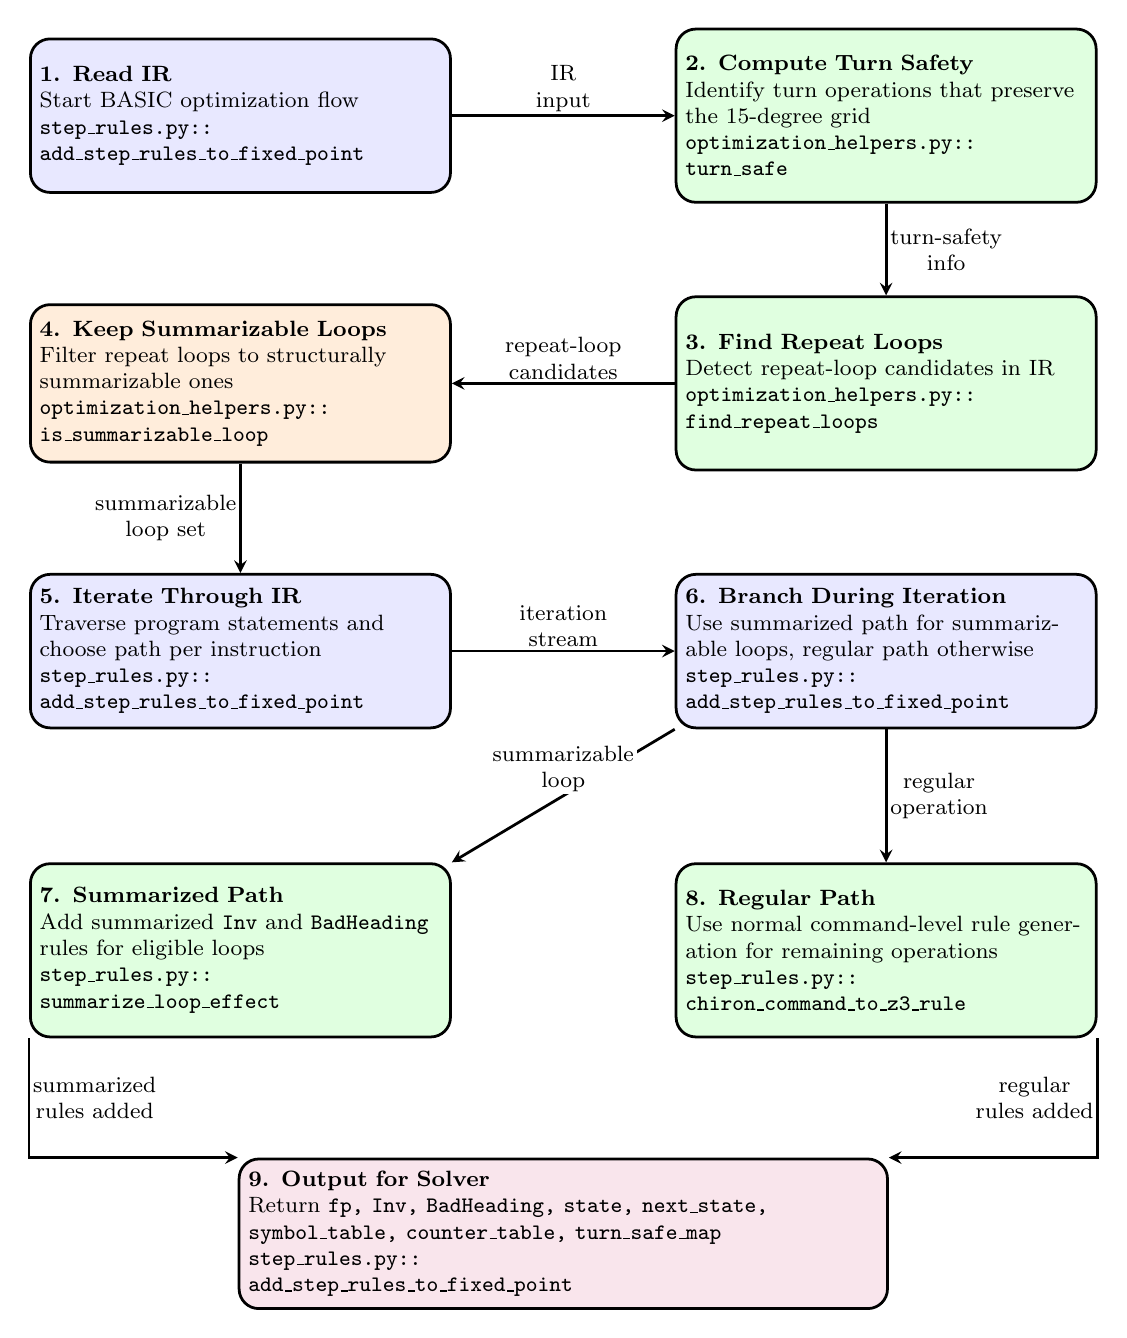
\begin{tikzpicture}[>=stealth, line width=1pt, font=\footnotesize]
\tikzset{
	opstage/.style={draw, rounded corners=2.5mm, align=left, text width=5.1cm, minimum height=1.95cm, fill=blue!9},
	opheavy/.style={draw, rounded corners=2.5mm, align=left, text width=5.1cm, minimum height=2.2cm, fill=green!12},
	opgate/.style={draw, rounded corners=2.5mm, align=left, text width=5.1cm, minimum height=2.0cm, fill=orange!14},
	opout/.style={draw, rounded corners=2.5mm, align=left, text width=8.0cm, minimum height=1.9cm, fill=purple!10}
}

\node[opstage] (o1) at (0,0)
{\textbf{1. Read IR}\\
Start BASIC optimization flow\\
\texttt{step\_rules.py::\\add\_step\_rules\_to\_fixed\_point}};

\node[opheavy] (o2) at (8.2,0)
{\textbf{2. Compute Turn Safety}\\
Identify turn operations that preserve the 15-degree grid\\
\texttt{optimization\_helpers.py::\\turn\_safe}};

\node[opheavy] (o3) at (8.2,-3.4)
{\textbf{3. Find Repeat Loops}\\
Detect repeat-loop candidates in IR\\
\texttt{optimization\_helpers.py::\\find\_repeat\_loops}};

\node[opgate] (o4) at (0.0,-3.4)
{\textbf{4. Keep Summarizable Loops}\\
Filter repeat loops to structurally summarizable ones\\
\texttt{optimization\_helpers.py::\\is\_summarizable\_loop}};

\node[opstage] (o5) at (0,-6.8)
{\textbf{5. Iterate Through IR}\\
Traverse program statements and choose path per instruction\\
\texttt{step\_rules.py::\\add\_step\_rules\_to\_fixed\_point}};

\node[opstage] (o6) at (8.2,-6.8)
{\textbf{6. Branch During Iteration}\\
Use summarized path for summarizable loops, regular path otherwise\\
\texttt{step\_rules.py::\\add\_step\_rules\_to\_fixed\_point}};

\node[opheavy] (o7) at (0,-10.6)
{\textbf{7. Summarized Path}\\
Add summarized \texttt{Inv} and \texttt{BadHeading} rules for eligible loops\\
\texttt{step\_rules.py::\\summarize\_loop\_effect}};

\node[opheavy] (o8) at (8.2,-10.6)
{\textbf{8. Regular Path}\\
Use normal command-level rule generation for remaining operations\\
\texttt{step\_rules.py::\\chiron\_command\_to\_z3\_rule}};

\node[opout] (o9) at (4.1,-14.2)
{\textbf{9. Output for Solver}\\
Return \texttt{fp, Inv, BadHeading, state, next\_state, symbol\_table, counter\_table, turn\_safe\_map}\\
\texttt{step\_rules.py::\\add\_step\_rules\_to\_fixed\_point}};

\draw[->] (o1.east) -- node[above, align=center, fill=white, inner sep=1pt] {IR\\input} (o2.west);
\draw[->] (o2.south) -- node[right, align=center, fill=white, inner sep=1pt] {turn-safety\\info} (o3.north);
\draw[->] (o3.west) -- node[above, align=center, fill=white, inner sep=1pt] {repeat-loop\\candidates} (o4.east);
\draw[->] (o4.south) -- node[left, align=center, fill=white, inner sep=1pt] {summarizable\\loop set} (o5.north);
\draw[->] (o5.east) -- node[above, align=center, fill=white, inner sep=1pt] {iteration\\stream} (o6.west);

\draw[->] (o6.south west) -- node[above, align=center, fill=white, inner sep=1pt] {summarizable\\loop} (o7.north east);
\draw[->] (o6.south) -- node[right, align=center, fill=white, inner sep=1pt] {regular\\operation} (o8.north);

\draw[->] (o7.south west) |- node[pos=0.25, right, align=center, fill=white, inner sep=1pt] {summarized\\rules added} (o9.north west);
\draw[->] (o8.south east) |- node[pos=0.25, left, align=center, fill=white, inner sep=1pt] {regular\\rules added} (o9.north east);

\end{tikzpicture}
\caption{BASIC optimization workflow: read IR, compute turn safety, detect and filter repeat loops to summarizable loops, then during iteration emit summarized \texttt{Inv}/\texttt{BadHeading} rules for eligible loops and regular rules for other operations.}
\label{fig:optimization_workflow}
\end{figure}

New optimazation layer with two supported modes. In
\texttt{OptimizationLevel.BASIC}, the verifier computes a static environment over
IR control-flow to detect turn operations that provably preserve the 15-degree
grid (\texttt{turn\_safe}). It also detects canonical repeat-loop shapes through
\texttt{find\_repeat\_loops(\ldots)} and admits only structurally safe loops via
\texttt{is\_summarizable\_loop(\ldots)}.

For those loops, \texttt{step\_rules.py} synthesizes a summarized transition from
loop-entry PC directly to loop-exit PC and emits any required summarized
\texttt{BadHeading} obligations. For non-summarized code, the original
instruction-wise rule generation remains active. This preserves soundness while
reducing rule count and symbolic clutter on common deterministic repeat patterns.

An additional semantic tightening is that movement trig handling was upgraded
from interval over-approximation buckets to exact 15-degree lookup values
(\texttt{cos\_sin\_exact\_z3}), aligning the transition encoding with the new
heading-grid reasoning.
The \texttt{OptimizationLevel.NONE} mode bypassed the optimization pipeline and performs standard verification.
See \autoref{fig:optimization_workflow} for a visual overview of the optimization flow.

\subsection*{Implementation Details: Property Scope}
\noindent\textit{\small File: \texttt{CHC-Verification/safety\_properties.py}}

The new \texttt{property\_scope} input supports \texttt{"all"} and
\texttt{"terminating"}. For terminating-only checks, the implementation:

\begin{enumerate}[leftmargin=1.5em]
	\item computes terminal PC as \texttt{len(ir)};
	\item checks reachability of terminating states using
	\texttt{Exists(vars, Inv(state) \& term\_guard)};
	\item returns \texttt{UNKNOWN} early if termination is unreachable/unknown;
	\item conjoins \texttt{term\_guard} into assumptions for all property queries.
\end{enumerate}

This keeps a single property-checking loop while changing the semantic domain of verification in a principled way.

\subsection*{Implementation Details: Heading-grid Safety Check}
\textit{
	Files:
	\begin{enumerate}
		\item \texttt{CHC-Verification/z3\_fixed\_point.py}
		\item \texttt{CHC-Verification/init\_fixed\_point.py}
		\item \texttt{CHC-Verification/step\_rules.py}
		\item \texttt{CHC-Verification/heading\_grid.py}
	\end{enumerate}
}

\begin{figure}[h]
\centering
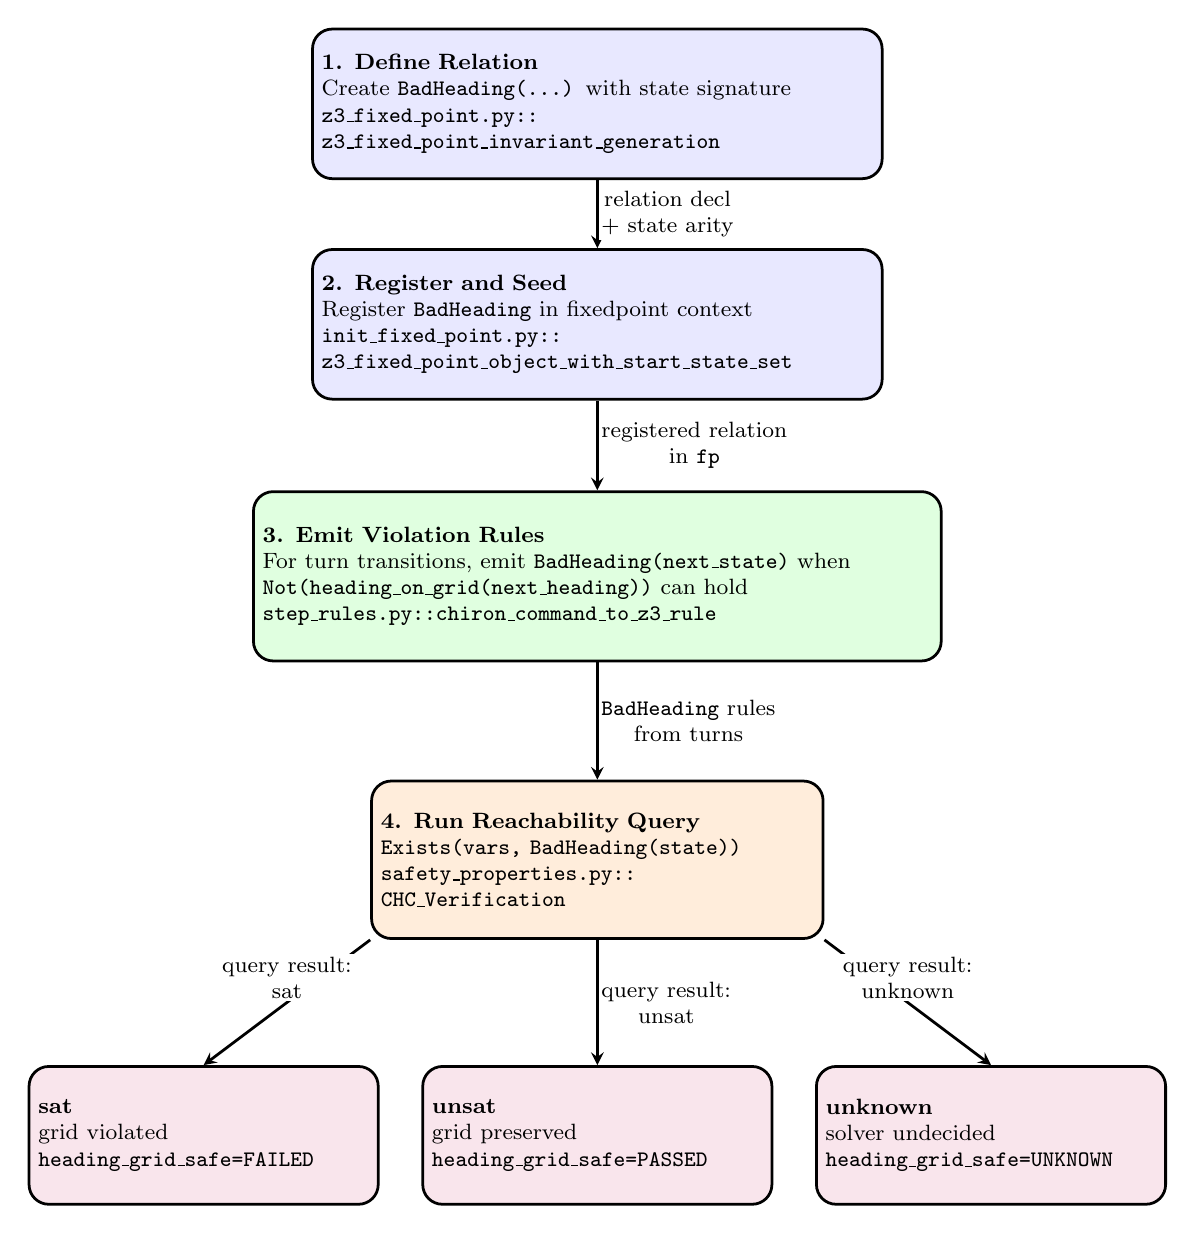
\begin{tikzpicture}[>=stealth, line width=1pt, font=\footnotesize]
\tikzset{
	bhstage/.style={draw, rounded corners=2.5mm, align=left, text width=7.0cm, minimum height=1.9cm, fill=blue!9},
	bhheavy/.style={draw, rounded corners=2.5mm, align=left, text width=8.5cm, minimum height=2.15cm, fill=green!12},
	bhquery/.style={draw, rounded corners=2.5mm, align=left, text width=5.5cm, minimum height=2.0cm, fill=orange!14},
	bhresult/.style={draw, rounded corners=2.5mm, align=left, text width=4.2cm, minimum height=1.75cm, fill=purple!10}
}

\node[bhstage] (b1) at (0,0)
{\textbf{1. Define Relation}\\
Create \texttt{BadHeading(\ldots)} with state signature\\
\texttt{z3\_fixed\_point.py::\\z3\_fixed\_point\_invariant\_generation}};

\node[bhstage] (b2) at (0,-2.8)
{\textbf{2. Register and Seed}\\
Register \texttt{BadHeading} in fixedpoint context\\
\texttt{init\_fixed\_point.py::\\z3\_fixed\_point\_object\_with\_start\_state\_set}};

\node[bhheavy] (b3) at (0,-6.0)
{\textbf{3. Emit Violation Rules}\\
For turn transitions, emit \texttt{BadHeading(next\_state)} when\\
\texttt{Not(heading\_on\_grid(next\_heading))} can hold\\
\texttt{step\_rules.py::chiron\_command\_to\_z3\_rule}};

\node[bhquery] (b4) at (0,-9.6)
{\textbf{4. Run Reachability Query}\\
\texttt{Exists(vars, BadHeading(state))}\\
\texttt{safety\_properties.py::\\CHC\_Verification}};

\node[bhresult] (bsat) at (-5.0,-13.1)
{\textbf{sat}\\
grid violated\\
\texttt{heading\_grid\_safe=FAILED}};

\node[bhresult] (bunsat) at (0,-13.1)
{\textbf{unsat}\\
grid preserved\\
\texttt{heading\_grid\_safe=PASSED}};

\node[bhresult] (bunk) at (5.0,-13.1)
{\textbf{unknown}\\
solver undecided\\
\texttt{heading\_grid\_safe=UNKNOWN}};

\draw[->] (b1.south) -- node[right, align=center, fill=white, inner sep=1pt] {relation decl\\+ state arity} (b2.north);
\draw[->] (b2.south) -- node[right, align=center, fill=white, inner sep=1pt] {registered relation\\in \texttt{fp}} (b3.north);
\draw[->] (b3.south) -- node[right, align=center, fill=white, inner sep=1pt] {\texttt{BadHeading} rules\\from turns} (b4.north);

\draw[->] (b4.south west) -- node[above, align=center, fill=white, inner sep=1pt] {query result:\\ sat} (bsat.north);
\draw[->] (b4.south) -- node[right, align=center, fill=white, inner sep=1pt] {query result:\\ unsat} (bunsat.north);
\draw[->] (b4.south east) -- node[above, align=center, fill=white, inner sep=1pt] {query result:\\ unknown} (bunk.north);

\end{tikzpicture}

\caption{BadHeading workflow for proving whether heading remains on the 15-degree grid and mapping query outcomes to verification status.}
\label{fig:badheading_workflow}
\end{figure}

The new pipeline introduces a dedicated relation
\texttt{BadHeading(\ldots)} at the invariant signature level and registers it in the fixedpoint context. Transition rules for turn commands can emit
\texttt{BadHeading} consequences whenever \texttt{Not(heading\_on\_grid(next\_heading))}
is reachable, see \autoref{fig:badheading_workflow} for the workflow.

At API level, when checking is requested, the verifier queries
\texttt{Exists(vars, BadHeading(state))}. The result semantics are:
\texttt{sat -> heading\_grid\_safe = FAILED (overall UNKNOWN)},
\texttt{unsat -> heading\_grid\_safe = PASSED (continue)},
\texttt{unknown -> heading\_grid\_safe = UNKNOWN (overall UNKNOWN)}.

This turns an implicit modeling assumption into an explicit proof obligation,
improving interpretability of trig-sensitive verification outcomes.

\subsection*{Implementation Details: Heading-grid Hints}
\noindent\textit{\small File: \texttt{CHC-Verification/safety\_properties.py}}

Hints are parsed as a \texttt{StrEnum} with values
\texttt{check\_heading\_always\_on\_grid} and
\texttt{heading\_on\_grid\_always}. The implementation validates hint type and
value, then applies a precedence rule:

\begin{itemize}[leftmargin=1.5em]
	\item if \texttt{heading\_on\_grid\_always} is present, the solver skips the
	heading-grid query and directly injects \texttt{heading\_on\_grid(state[3])}
	into assumptions;
	\item otherwise, if \texttt{check\_heading\_always\_on\_grid} is present,
	the explicit \texttt{BadHeading} query is performed.
\end{itemize}

In \texttt{OptimizationLevel.BASIC}, if static analysis proves every turn is safe
(\texttt{is\_all\_turn\_safe}), the heading-grid check short-circuits to PASSED,
avoiding unnecessary solver effort.

\subsection*{API Usage Guide}

The expected calling pattern is:

\begin{lstlisting}[style=terminal, language=python]
from safety_properties import CHC_Verification
from variable_name_detection_in_IR import OptimizationLevel

class UserProperty:
	def __init__(self, name, expr):
		self.name = name
		self.expr = expr

props = [UserProperty("x_nonneg", "x >= 0")]

result = CHC_Verification(
	"correctness_tests/programs/loop_accum.tl",
	"default",
	props,
	property_scope="all",
	hints=["check_heading_always_on_grid"],
	timeout_ms=60_000,
	optimization_level=OptimizationLevel.BASIC,
)

print("Result:", result.status)
print("Heading Grid Safe:", result.heading_grid_safe)
print("Build Time:", result.build_time)
print("Solve Times:", result.solve_times)
\end{lstlisting}

Operational notes:
\begin{itemize}[leftmargin=1.5em]
	\item Use \texttt{specific} mode with a parameter dictionary string
	(e.g., \texttt{"{'x': 10}"});
	\item Use \texttt{property\_scope="terminating"} only when termination-focused
	properties are intended;
	\item Prefer \texttt{check\_heading\_always\_on\_grid} unless the program is known to be heading-grid safe or the check is not relevant, as provides a good balance of soundness and performance.
\end{itemize}